\documentclass{beamer}

\usepackage{beamerthemeshadow}
\usepackage{color}
\usepackage{verbatim}
\usepackage{tikz}
%\usepackage[normalem]{ulem}
%\usepackage{wrapfig}

\mode<presentation>
{
 \usetheme{Warsaw} %%% Change later
\usecolortheme{dove}

%gets rid of bottom navigation bars
\setbeamertemplate{footline}[page number]{}

  \setbeamercovered{transparent}
  % or whatever (possibly just delete it)
}


\usepackage{graphicx}

\usepackage{amssymb,soul}

\usepackage{hyperref}

\definecolor{myblue}{rgb}{0, 0, 0.9}

\definecolor{mygreen}{rgb}{0,0.6,0}

\definecolor{mymagenta}{rgb}{0.9, 0, 0.9}

\definecolor{myred}{rgb}{0.9,0,0}

\definecolor{mygray}{rgb}{0.8,0.8,0.8}

\definecolor{mydark}{rgb}{0.4, 0.4, 0.4}

\definecolor{myblack}{rgb}{0,0,0}

\newcommand{\msblue}[1]{{\color{myblue} #1}}

\newcommand{\msmagenta}[1]{{\color{mymagenta} #1}}

\newcommand{\msred}[1]{{\color{myred} #1}}

\newcommand{\msgreen}[1]{{\color{mygreen} #1}}

\newcommand{\msgray}[1]{{\color{mygray} #1}}

\newcommand{\msdark}[1]{{\color{mydark} #1}}

\newcommand{\msblack}[1]{{\color{myblack} #1}}

\newcommand{\relu}{\mbox{\bf ReLU}}

\begin{document}

\title{Higher-order neuromorphic computations with linear streams}
\author{\bf Mishka (Michael Bukatin)}
\date[]  
{\footnotesize Dataflow Matrix Machines project\\[2ex]
\href{https://anhinga.github.io}{\tt https://anhinga.github.io}\\[6ex] 
CCC 2020: Continuity, Computability, Constructivity –\\ From Logic to Algorithms\\[2ex]
September 3, 2020
}

\begin{frame}
  \titlepage
\end{frame}

\begin{frame}

I overview work done in 2012-2020.\\[2ex]

Most of this work is done in a series of research collaborations with Steve Matthews, Ralph Kopperman, Andrey Radul, Jon Anthony.\\[2ex]

{\bf I am looking for collaborators.}\\[2ex]

e-mail: {\tt bukatin@cs.brandeis.edu}\\[2ex]

these slides are linked from \href{https://www.cs.brandeis.edu/~bukatin/dmm\_next.html}{\tt https://www.cs.brandeis.edu/$\sim$bukatin/dmm\_next.html}

\end{frame}

\begin{frame}

\begin{enumerate}

  \item How to make vector spaces from Scott domains

  \begin{itemize}
      \item \msgray{Add overdefined elements (to cancel partially defined elements)}
      \item \msgray{Obtain bicontinuous domains with two Scott topologies}
      \item \msgray{Obtain rich mathematical landscape}
  \end{itemize}

  \vspace{2ex}

  \item Computing with vector-like streams

  \begin{itemize}
      \item \msgray{Natural degree of generality for neural model of computation}
      \item \msgray{Continuously deformable general-purpose programs}
      \item \msgray{Neural machines which can fluently modify themselves}

  \end{itemize}

  \vspace{2ex}

  \item Interplay between 1 and 2, and open problems

\end{enumerate}

\end{frame}

\begin{frame}

\begin{enumerate}

  \item How to make vector spaces from Scott domains

  \begin{itemize}
      \item Add overdefined elements (to cancel partially defined elements)
      \item Obtain bicontinuous domains with two Scott topologies
      \item Obtain rich mathematical landscape
  \end{itemize}

  \vspace{2ex}

  \item Computing with vector-like streams

  \begin{itemize}
      \item \msgray{Natural degree of generality for neural model of computation}
      \item \msgray{Continuously deformable general-purpose programs}
      \item \msgray{Neural machines which can fluently modify themselves}

  \end{itemize}

  \vspace{2ex}

  \item Interplay between 1 and 2, and open problems

\end{enumerate}

\end{frame}

\begin{frame}

\begin{enumerate}

  \item How to make vector spaces from Scott domains

  \begin{itemize}
      \item Add overdefined elements (to cancel partially defined elements)
      \item Obtain bicontinuous domains with two Scott topologies
      \item Obtain rich mathematical landscape
  \end{itemize}

  \vspace{2ex}

  \item Computing with vector-like streams

  \begin{itemize}
      \item Natural degree of generality for neural model of computation
      \item Continuously deformable general-purpose programs
      \item Neural machines which can fluently modify themselves

  \end{itemize}

  \vspace{2ex}

  \item Interplay between 1 and 2, and open problems

\end{enumerate}

\end{frame}

\section{Partial inconsistency landscape}

\begin{frame}
    The essence of problem, consider negation in interval numbers:\\[2ex]

    $[5, 7] + [-7, -5] = [-2, 2] \sqsubset [0, 0]$.\\[2ex]

    \msgray{To fix this: allow {\bf pseudosegments},\\ where the endpoints are in the ``wrong" order:\\[2ex]

    $[7, 5], [-5, -7],$ etc.\\[2ex]

    Then we get {\bf true negation} and an {\bf abelian group}.}

\end{frame}

\begin{frame}
    The essence of problem, consider negation in interval numbers:\\[2ex]

    $[5, 7] + [-7, -5] = [-2, 2] \sqsubset [0, 0]$.\\[2ex]

    To fix this: allow {\bf pseudosegments},\\ where the endpoints are in the ``wrong" order:\\[2ex]

    $[7, 5], [-5, -7],$ etc.\\[2ex]

    \msgray{Then we get {\bf true negation} and an {\bf abelian group}.}

\end{frame}

\begin{frame}
    The essence of problem, consider negation in interval numbers:\\[2ex]

    $[5, 7] + [-7, -5] = [-2, 2] \sqsubset [0, 0]$.\\[2ex]

    To fix this: allow {\bf pseudosegments},\\ where the endpoints are in the ``wrong" order:\\[2ex]

    $[7, 5], [-5, -7],$ etc.\\[2ex]

    Then we get {\bf true negation} and an {\bf abelian group}.

\end{frame}

\begin{frame}

  \frametitle{Multiple rediscoveries}

Known under various names: Kaucher interval arithmetic, directed interval arithmetic, generalized
interval arithmetic, modal interval arithmetic, interval algebraic extensions, etc.\\[2ex]

First mention we know: M. Warmus,  Calculus of Approximations. Bull. Acad. Pol. Sci., Cl. III, 4(5): 253-259, 1956,
\url{http://www.cs.utep.edu/interval-comp/warmus.pdf}\\[2ex]

A comprehensive repository
of literature on the subject is maintained by Evgenija Popova: The Arithmetic on Proper \& Improper Intervals (a Repository of Literature on Interval Algebraic Extensions),
\url{http://www.math.bas.bg/~epopova/directed.html}



\end{frame}

\begin{frame}

  \frametitle{From Cartesian to Hasse representation}

{\center 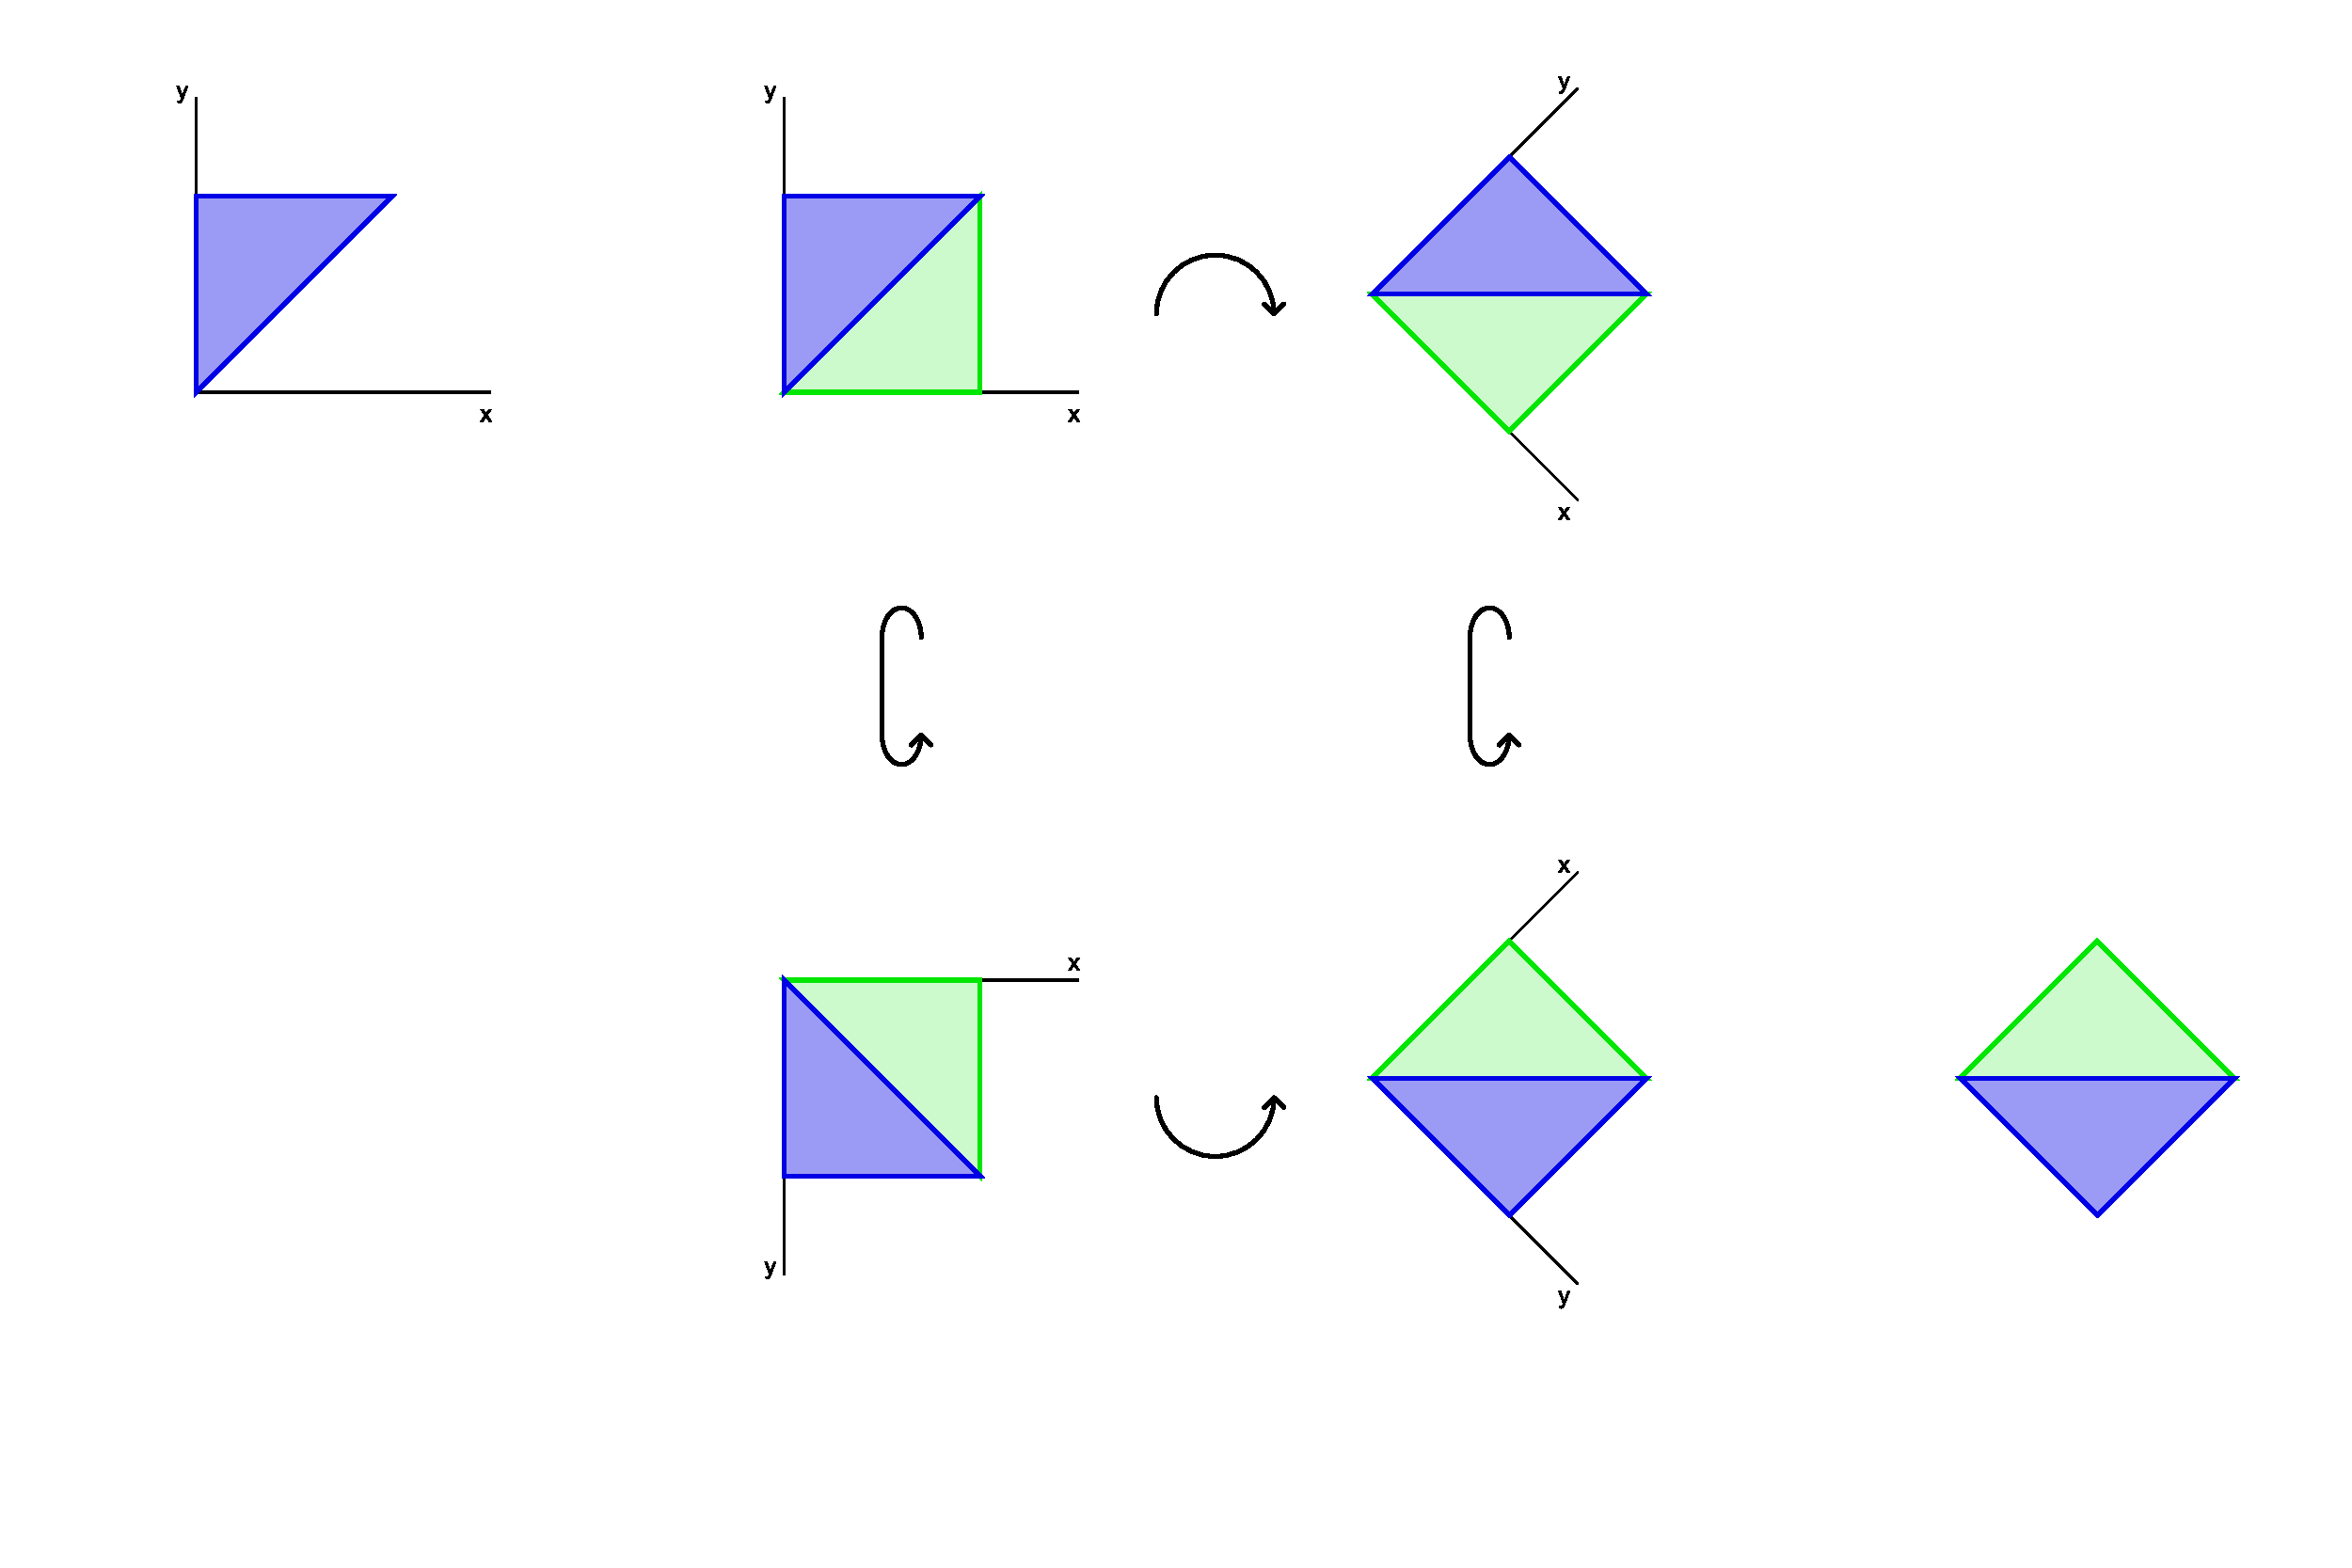
\includegraphics[height=72mm]{to_hasse.pdf}}


\end{frame}

\begin{frame}

  \frametitle{Bicontinuous domains}

K.~Keimel.  Bicontinuous domains and some old problems in domain theory. {\em Electronic Notes in Theoretical Computer Science}, {\bf 257}:35-54, 2009\\[2ex]

\begin{itemize}
  \item Two Scott topologies, not one.
  \item Order-reversing involution.
  \item Computations can be done via either of these topologies.
  \item Use involution to switch between them?
  \item Classical logic (classical treatment of negation)?
\end{itemize} 

\end{frame}

\begin{frame}

  \frametitle{Partial inconsistency landscape}


\begin{itemize}

\item{Negative distance/probability/degree of set membership}

\item{Bilattices}

\item{Partial inconsistency}

\item{Non-monotonic inference}

\item{Bitopology}

\item{$x = (x \wedge 0) + (x \vee 0)$ or $x = (x \wedge \bot) \sqcup (x \vee \bot)$ }

\item{\msblue{Scott domains tend to become embedded into vector spaces}}

\item{Modal and paraconsistent logic and possible world models}

\item{Bicontinuous domains}

\item{The domain of arrows, $D^{Op}\times D$ or $C^{Op}\times D$}

\end{itemize}

\end{frame}

\begin{frame}
  M.~Bukatin, S.~Matthews.
Linear Models of Computation and Program Learning. In G.~Gottlob, G.~Sutcliffe, A.~Voronkov, editors,
GCAI 2015, {\em EasyChair Proceedings in Computing}, {\bf 36}, 66-78.
\href{https://easychair.org/publications/paper/Q4lW}{\tt\footnotesize https://easychair.org/publications/paper/Q4lW}\\[6ex]

M.~Bukatin.
{\em Using streams of probabilistic samples in neural machines.} January 2020.
\href{https://github.com/anhinga/2020-notes/tree/master/research-notes}{\tt\footnotesize https://github.com/anhinga/2020-notes/tree/master/research-notes}


\end{frame}


\section{Dataflow matrix machines (DMMs)}

\begin{frame}
   We have rich mathematics of bicontinuous domains, which seems likely to be suitable to define denotational 
   {\bf vector semantics}
   of programming languages.\\[2ex]

   The natural question then arises: can one program in terms of vector-like elements?\\[2ex]

   That is, can one define {\bf operational semantics} (implementation) in terms of vector-like elements?\\[2ex]

   More specifically, is programming with {\bf linear streams} (streams which can be
   combined with numerical coefficients) sufficient for general-purpose programming?
\end{frame}

\begin{frame}
   We'll be talking about programming in {\bf dataflow style} (or, in more modern terms, in
   {\bf functional reactive style}).\\[2ex]

   We know that short {\bf probabilistic programs} are very expressive.\\[2ex]

   So are short {\bf functional reactive animations programs} generalizing digital audio
   synthesis by composition of unit generators, see e.g.
   \href{https://youtu.be/fEWcg\_A5UZc}{\tt https://youtu.be/fEWcg\_A5UZc}\\[2ex]

   Our present collection of programming techniques and examples is diverse enough to support the claim that
this formalism is sufficiently expressive for general purpose programming:\\[1ex]
   M.~Bukatin.
{\em Overview of programming techniques and examples in DMM literature.} January 2020.\\
\href{https://github.com/anhinga/2020-notes/tree/master/programming-overview}
{\tt\scriptsize https://github.com/anhinga/2020-notes/tree/master/programming-overview}
\end{frame}

\begin{frame}
   But can one do higher-order programming in this style? And can one {\bf deform the resulting programs
in a continuous fashion}?\\[2ex]

   It turns out that the answer is yes, if one agrees to {\bf interleave linear and non-linear
transformations of linear streams}.\\[2ex]

   Here we came from the viewpoint of stream-oriented programming.\\[2ex]

   One can also arrive at the same result from the viewpoint of {\bf recurrent neural networks}.\\[2ex]

  The essence of neural model of computations is that linear and non-linear computations are interleaved.  So, the natural degree of generality for neuromorphic computations is to work not with streams of numbers, but with arbitrary  
{\bf linear streams}.

  

\end{frame}

\begin{frame}

  \frametitle{\msmagenta{Dataflow matrix machines (DMMs)}}

DMMs: a novel class of {\bf neural machines}.\\[2ex]

They use arbitrary {\bf linear streams} instead of streams of numbers.\\[2ex]


\begin{itemize}

\item {\bf Self-modification:} can fluently modify their own weights, connectivity patterns, and size;\\[2ex]

\item Highly expressive linear streams of V-values\\ (vector-like values based on nested dictionaries);\\[2ex]

\item Expressive enough to serve as a programming platform: functional reactive programming with\\ {\bf continuously deformable programs}.

\end{itemize}

\end{frame}




\begin{frame}

\frametitle{\msmagenta{Linear streams}}

The key feature of {\bf DMMs} compared to {\bf RNNs}:
         they use\\ {\bf linear streams} instead of streams of numbers.\\[2ex]

The following streams all support the pattern of alternating\\ linear and non-linear computations:\\[2ex]

\begin{itemize}

\item Streams of numbers\\[2ex]

\item Streams of vectors from fixed vector space $V$\\[2ex]

\item Linear streams: such streams that the notion of\\ {\bf linear combination of several streams} is defined.\\[3ex]

\end{itemize}






\end{frame}




\begin{frame}

\frametitle{Kinds of linear streams}

 Some examples:\\[1ex]


\begin{itemize}


\item Every vector space $V$ gives rise to the corresponding kind of linear streams
(streams of vectors from that space)\\[2ex]

\item \msmagenta{Every measurable space $X$ gives rise to the space of\\ {\bf streams of
probabilistic samples} drawn from $X$\\ and decorated with +/- signs\\
(linear combination is defined by a stochastic procedure)}\\[2ex]

\item Streams of images of a particular size (that is, animations)\\[2ex]

\item Streams of matrices; streams of multidimensional arrays\\[2ex]

\item \msmagenta{Streams of V-values based on nested maps (instead of S-expressions)}\\[2ex]



\end{itemize}

\end{frame}












\section{V-values and variadic neurons}







\subsection{Vectors based on nested maps}


\begin{frame}

  \frametitle{\msmagenta{V-values: vector space based on nested dictionaries}}


V-values play the role of Lisp S-expressions in this formalism.\\[3ex]


We want a vector space.\\[3ex]

Take prefix trees with numerical leaves\\ implemented as nested dictionaries.\\[3ex]

We call them {\bf V-values}
(``vector-like values").\\[3ex]


\end{frame}







\begin{frame}

  \frametitle{\msmagenta{Example of a V-value: different ways to view it}}

\begin{columns}[T]
\begin{column}{0.5\textwidth}

\begin{tikzpicture}
  \clip (-3.0, -4.5) rectangle (3.0, 0.0);

  \draw[->](0, 0) -- (-1.8, -1)  node [below] {3.5};

  \draw[->](0, 0) -- (0, -1) node [midway,  below right] {:foo};

    \draw[->](0, -1) -- (0.5, -2) node[midway, below right] {\ :bar};

      \draw[->](0.5, -2) -- (0.5, -3) node [below] {7};

    \draw[->](0, -1) -- (-0.5, -2) node [below] {2};

  \draw[->](0, 0) -- (1.8, -1) node [midway, below  right] {\ \ \ \ \ \ :baz};

      \draw[->](1.8, -1) -- (1.8, -2) node [midway, below  right] {:foo};

      \draw[->](1.8, -2) -- (1.8, -3) node [midway, below  right] {:bar};      

      \draw[->](1.8, -3) -- (1.8, -4) node [below] {-4};
 

  \filldraw (1.8, -1) circle [radius=0.7pt]
                (1.8, -2) circle [radius=0.7pt]
                (1.8, -3) circle [radius=0.7pt]
                (0, -1) circle [radius=0.7pt]
                (0.5, -2) circle [radius=0.7pt];
  
 

\end{tikzpicture}
\end{column}
\begin{column}{0.5\textwidth}

\begin{itemize}

{\footnotesize

 \item 3.5 $\cdot$ ($\epsilon$) + 2 $\cdot$ (:foo) + \\ 7 $\cdot$ (:foo :bar) - 4 $\cdot$ (:baz :foo :bar)

 \item ($\leadsto$ 3.5) + (:foo $\leadsto$  2) +\\ (:foo $\leadsto$ :bar $\leadsto$ 7) +\\
          (:baz $\leadsto$ :foo $\leadsto$ :bar $\leadsto$ -4)


\msmagenta{
 \item {\tiny  scalar 3.5 + sparse 1D array \{{\tt d1[:foo]= 2}\} +\\[1.5ex] sparse 2D
matrix \{{\tt d2[:foo, :bar]= 7}\} +\\  sparse 3D array \{{\tt d3[:baz, :foo, :bar]= -4}\}}
}

 \item {\tt \{:number 3.5,\\ :foo \{:number 2, :bar 7\}, :baz \{:foo \{:bar -4\}\}\}}
          ({\tt :number} $\not\in L$)

}

\end{itemize}

\end{column}
\end{columns}

\end{frame}






\subsection{Variable arity}


\begin{frame}

  \frametitle{Dataflow matrix machines (our current implementation) based on
 streams of  V-values
 and
 variadic neurons}

$x_{f, n_f, i}^{t+1} = \sum_{g \in F} \sum_{n_g \in L} \sum_{o \in L} \msblue{w_{f, n_f, i;\, g, n_g, o}^t} * y_{g, n_g, o}^t$ {\small \msblue{(down movement)}}\\[2ex]

$y_{f, n_f}^{t+1} = f(x_{f, n_f}^{t+1})$ {\small \msgreen{(up movement)}}

\begin{tikzpicture}
  %\draw (-3.5, -2.0) rectangle (7.0, 2.0);
  \clip (-3.5, -2.0) rectangle (7.0, 2.0);

  \filldraw (-3.2,0) circle [radius=0.5pt]
                (-3.0,0)  circle [radius=0.5pt]
                (-3.4, 0) circle [radius=0.5pt]; 

\msgreen{\draw [->] (-2.6, -1.5) node[right] {\msmagenta{$x_{f, n_f}$}} -- (-2.6, 1.5) node [midway, above right] {$f$} node[right] {\msmagenta{$y_{f, n_f}$}};}

  \filldraw (0,0) circle [radius=0.5pt]
                (-0.2,0)  circle [radius=0.5pt]
                (0.2, 0) circle [radius=0.5pt];

\msgreen{\draw [->] (0.6, -1.5) node[right] {\msmagenta{$x_{g, n_g}$}} -- (0.6, 1.5) node [midway, above right] {$g$} node[right] {\msmagenta{$y_{g, n_g}$}};}

  \filldraw (3.2,0) circle [radius=0.5pt]
                (3.0,0)  circle [radius=0.5pt]
                (3.4, 0) circle [radius=0.5pt]; 


 \msblue{ \draw [->, very thick] (1.1, 1.1) .. controls (5.5, 4.3) and (5.5, -4.0) .. (1.1, -0.8)  node [midway, right] {{\bf W}};}

  \foreach \y in {-1.0, 1.0}
    {

      \draw [densely dotted] (0.45, \y+0.15) ellipse [x radius=100pt, y radius=4pt];

     \foreach \x in {-1.0, 2.2}
       {

        \foreach \d in {-0.4, -0.15, 0.1}
           {
               \msmagenta{\draw(\x-0.15, \y + 0.45) -- (\x+\d, \y+0.15); 
               \draw (\x+\d, \y + 0.15) -- (\x+\d-0.08, \y-0.15);
               \draw (\x+\d, \y + 0.15) -- (\x+\d+0.08, \y-0.15);
               \filldraw (\x+0.5*\d-0.05, \y-0.25) circle [radius=0.2pt];
               \filldraw (\x+0.5*\d+0.5, \y+0.15) circle [radius=0.2pt];}
           }
       } 
     }
 
\end{tikzpicture}

\end{frame}

\section{Programming patterns and self-referential facilities}




\begin{frame}

  \frametitle{\msmagenta{DMMs: programming with powerful neurons}}

Powerful variadic neurons and streams of V-values $\Rightarrow$ a much more expressive formalism
 than networks based on streams of numbers.\\[2ex]

Many tasks can be accomplished by \msmagenta{compact DMM networks},\\
 where {\bf single neurons function as layers or modules}.

\hrulefill

\begin{itemize}

\item Accumulators and memory

\item Multiplicative constructions and ``fuzzy if"

\item Sparse vectors

\item Data structures

\item Self-referential facilities

\end{itemize}






\end{frame}

\begin{frame}

  \frametitle{\msmagenta{Accumulators and memory}}

\begin{tikzpicture}
   \clip (-2.0, -2.0) rectangle (7.0, 2.0);




  \filldraw (0,0) circle [radius=0.5pt]
                (-0.2,0)  circle [radius=0.5pt]
                (0.2, 0) circle [radius=0.5pt];

\msgreen{\draw [->] (0.6, -1.5) node[right] {\msblack{$x_{{\tt plus}, {\tt :my\mbox{\footnotesize -}neuron}}$}} -- 
                    (0.6, 1.5) node [midway, above right] {\tt plus} node[right]
                    {\msblack{$y_{{\tt plus}, {\tt :my\mbox{\footnotesize -}neuron}}$}};}

  \filldraw (3.2,0) circle [radius=0.5pt]
                (3.0,0)  circle [radius=0.5pt]
                (3.4, 0) circle [radius=0.5pt]; 


 \msblue{\draw [->] (1.9, 1.1) .. controls (5.5, 4.3) and (5.5, -4.0) .. (2.15, -0.85)  node [midway, left] {{1.0}};

  \draw [->] (1.7, -0.2) -- (1.5, -0.9);
  \filldraw (1.5, -0.25) circle [radius=0.2pt];
  \filldraw (1.6, -0.25) circle [radius=0.2pt];
  \filldraw (1.4, -0.25) circle [radius=0.2pt];
  \draw [->] (1.3, -0.2) node [left] {{\tiny updates from other neurons}} -- (1.5, -0.8);}


  \foreach \y in {-1.0}
    {

      \draw [densely dotted] (1.0, \y+0.15) ellipse [x radius=80pt, y radius=5pt];

     \foreach \x in {2.0}
       {

        \foreach \d in {-0.4}
           {
               \draw(\x-0.15, \y + 0.45) -- (\x+\d, \y+0.15) node [left] {\scriptsize{\tt :delta}}; 
               \draw (\x+\d, \y + 0.15) -- (\x+\d-0.08, \y-0.15);
               \draw (\x+\d, \y + 0.15) -- (\x+\d+0.08, \y-0.15);
               \filldraw (\x+0.5*\d-0.05, \y-0.25) circle [radius=0.2pt];
               %\filldraw (\x+0.5*\d+0.5, \y+0.15) circle [radius=0.2pt];
           }
       \foreach \d in {0.1}
           {
               \draw(\x-0.15, \y + 0.45) -- (\x+\d, \y+0.15) node [right] {\scriptsize{\tt :accum}}; 
               \draw (\x+\d, \y + 0.15) -- (\x+\d-0.08, \y-0.15);
               \draw (\x+\d, \y + 0.15) -- (\x+\d+0.08, \y-0.15);
               \filldraw (\x+0.5*\d-0.05, \y-0.25) circle [radius=0.2pt];
               %\filldraw (\x+0.5*\d+0.5, \y+0.15) circle [radius=0.2pt];
           }
        \foreach \d in {-0.4, -0.15, 0.1}
           {
              \filldraw (\x+0.5*\d-0.05, \y-0.25) circle [radius=0.2pt];
           }
       } 
     }

  \foreach \y in {0.9}
    {

      \draw [densely dotted] (1.0, \y+0.15) ellipse [x radius=80pt, y radius=5pt];

     \foreach \x in {2.0}
       {

        \foreach \d in {-0.15}
           {
               \draw(\x-0.15, \y + 0.45) -- (\x+\d, \y+0.15) node [right] {\scriptsize{\tt :single}}; 
               \draw (\x+\d, \y + 0.15) -- (\x+\d-0.08, \y-0.15);
               \draw (\x+\d, \y + 0.15) -- (\x+\d+0.08, \y-0.15);
 
               %\filldraw (\x+0.5*\d+0.5, \y+0.15) circle [radius=0.2pt];
           }
        \foreach \d in {-0.4, -0.15, 0.1}
           {
              \filldraw (\x+0.5*\d-0.05, \y-0.25) circle [radius=0.2pt];
           }
       } 
     }
 
\end{tikzpicture}

In this implementation, activation function \msgreen{\footnotesize \tt plus} adds V-values from 
{\footnotesize\tt :accum} and {\footnotesize\tt :delta}
together and places the result into {\footnotesize\tt :single}.

\end{frame}


\subsection{Sparse vectors}



\begin{frame}

  \frametitle{Sparse vectors of high or infinite dimension}

Example:  a neuron accumulating count of words in a given text.\\[2ex]

The dictionary mapping words to their respective counts is an infinite-dimensional vector
with a finite number of non-zero elements.\\[2ex]

\msmagenta{\Large $\bullet$} Don't need a neuron for each coordinate of our vector space.\\[2ex]

 \msmagenta{\Large $\bullet$} Don't have an obligation to reduce dimension by embedding.

\end{frame}





\subsection{Data structures}





\begin{frame}

  \frametitle{Streams of immutable \msmagenta{data structures}}

One can represent {\bf lists, matrices, graphs,} and so on\\ via nested dictionaries.\\[3ex]


It is natural to use streams of immutable V-values in the implementations of DMMs.\\[3ex]

The DMM architecture is friendly towards algorithms working with immutable data structures in
the spirit of functional programming.\\[3ex]

But more imperative styles can be accommodated as well.

\end{frame}





\subsection{Self-referential facilities}





\begin{frame}

  \frametitle{\msmagenta{Self-referential facilities (easy in DMMs)}}

It is easy to represent the network matrix {\bf W} as a V-value.\\[3ex]

Emit the stream
of network matrices from neuron {\tt Self}.\\[3ex]

Use the most recent V-value from that stream
as the network matrix {\bf W} during the
next ``down movement".\\[3ex]

This mechanism allows a DMM network to 
{\bf modify its own weights, topology, and size}
while it is running.

\end{frame}


\begin{frame}

  \frametitle{\msmagenta{Self-referential facilities (easy in DMMs)}}

Our current implementation: {\tt Self} connected as an accumulator.\\[2ex]
It accumulates the value of the network matrix and
accepts additive updates from other neurons in the network.\\[2ex]

\begin{tikzpicture}
   \clip (-2.0, -2.0) rectangle (7.0, 2.0);




  \filldraw (0,0) circle [radius=0.5pt]
                (-0.2,0)  circle [radius=0.5pt]
                (0.2, 0) circle [radius=0.5pt];

  \msgreen{\draw [->] (0.6, -1.5) node[right] {\msblack{$x_{{\tt plus}, {\bf :Self}}$}} -- 
                    (0.6, 1.5) node [midway, above right] {{\tt plus}} node[right] {\msblack{$y_{{\tt plus}, {\bf :Self}}$}};}

  \filldraw (3.2,0) circle [radius=0.5pt]
                (3.0,0)  circle [radius=0.5pt]
                (3.4, 0) circle [radius=0.5pt]; 


  \msblue{\draw [->] (1.9, 1.1) .. controls (5.5, 4.3) and (5.5, -4.0) .. (2.15, -0.85)  node [midway, left] {{1.0}};

  \draw [->] (1.7, -0.2) -- (1.5, -0.9);
  \filldraw (1.5, -0.25) circle [radius=0.2pt];
  \filldraw (1.6, -0.25) circle [radius=0.2pt];
  \filldraw (1.4, -0.25) circle [radius=0.2pt];
  \draw [->] (1.3, -0.2) node [left] {{\tiny updates from other neurons}} -- (1.5, -0.8);}


  \foreach \y in {-1.0}
    {

      \draw [densely dotted] (1.0, \y+0.15) ellipse [x radius=80pt, y radius=5pt];

     \foreach \x in {2.0}
       {

        \foreach \d in {-0.4}
           {
               \draw(\x-0.15, \y + 0.45) -- (\x+\d, \y+0.15) node [left] {\scriptsize{\tt :delta}}; 
               \draw (\x+\d, \y + 0.15) -- (\x+\d-0.08, \y-0.15);
               \draw (\x+\d, \y + 0.15) -- (\x+\d+0.08, \y-0.15);
               \filldraw (\x+0.5*\d-0.05, \y-0.25) circle [radius=0.2pt];
               %\filldraw (\x+0.5*\d+0.5, \y+0.15) circle [radius=0.2pt];
           }
       \foreach \d in {0.1}
           {
               \draw(\x-0.15, \y + 0.45) -- (\x+\d, \y+0.15) node [right] {\scriptsize{\tt :accum}}; 
               \draw (\x+\d, \y + 0.15) -- (\x+\d-0.08, \y-0.15);
               \draw (\x+\d, \y + 0.15) -- (\x+\d+0.08, \y-0.15);
               \filldraw (\x+0.5*\d-0.05, \y-0.25) circle [radius=0.2pt];
               %\filldraw (\x+0.5*\d+0.5, \y+0.15) circle [radius=0.2pt];
           }
        \foreach \d in {-0.4, -0.15, 0.1}
           {
              \filldraw (\x+0.5*\d-0.05, \y-0.25) circle [radius=0.2pt];
           }
       } 
     }

  \foreach \y in {0.9}
    {

      \draw [densely dotted] (1.0, \y+0.15) ellipse [x radius=80pt, y radius=5pt];

     \foreach \x in {2.0}
       {

        \foreach \d in {-0.15}
           {
               \draw(\x-0.15, \y + 0.45) -- (\x+\d, \y+0.15) node [right] {\scriptsize{\bf :NetworkMatrix}}; 
               \draw (\x+\d, \y + 0.15) -- (\x+\d-0.08, \y-0.15);
               \draw (\x+\d, \y + 0.15) -- (\x+\d+0.08, \y-0.15);
 
               %\filldraw (\x+0.5*\d+0.5, \y+0.15) circle [radius=0.2pt];
           }
        \foreach \d in {-0.4, -0.15, 0.1}
           {
              \filldraw (\x+0.5*\d-0.05, \y-0.25) circle [radius=0.2pt];
           }
       } 
     }
 
\end{tikzpicture}

The most recent V-value at the {\footnotesize\tt :NetworkMatrix} output of\\ $y_{{\tt plus}, {\bf :Self}}$ neuron is used as \msblue{\bf W}.


\end{frame}

\section{Interplay between domains and DMMs; open problems}

\subsection{Interplay between domains and DMMs}

\begin{frame}

  \frametitle{Monotonic evolution of Warmus numbers by additions}

Consider $x \sqsubseteq  (x+x_1) \sqsubseteq  (x+x_1+x_2) \sqsubseteq \dots $\\[2ex]

Then every $x_i = [a_i, b_i]$ must be a pseudo-segment anti-approximating zero:\\[2ex]

$[0,0] \sqsubseteq [a_i,b_i]$, that is $b_i \leq 0 \leq a_i$.\\[2ex]

(\url{https://arxiv.org/abs/1610.00831}, Appendix A)

\end{frame}

\begin{frame}

  \frametitle{Rectifiers and quasi-metrics}

It was typical to use sigmoid non-linearities as activation functions in neural nets, but a few years ago people discovered that
{\bf ReLU} (rectified linear units) often work much better: $\relu(x) = max(0,x)$.\\[2ex]

This is an integral of the Heaviside step function. Lack of smoothness at 0 does not seem to
interfere with gradient methods, and otherwise it's nice when the derivatives are so simple.\\[2ex]

Our standard quasi-metrics on reals are closely related to ReLU:\\[2ex]

$q_1(x,y) = \relu(x-y) = q_2(y,x)$.\\[2ex]

(\url{https://arxiv.org/abs/1610.00831}, Appendix B)

\end{frame}

\subsection{Open problems}

\begin{frame}

   \frametitle{Open Problems}

   There are a bit more known connections between bicontinuous domains and DMM practice,
   but there should be much more.\\[2ex]

   Usually, we forget that programming with linear streams is related to bicontinuous domains,
   and we just use vector spaces,
   and we lose the potential hidden in the math of partial inconsistency.\\[2ex]

   We do have some hints. E.g. training of {\bf generative adversarial networks} does resemble computations
   with two Scott topologies and involution in spirit. One of the open problems is to investigate whether
   this connection can be formalized.
\end{frame}

\begin{frame}

   \frametitle{Open Problems}

   Both Klaus Keimel and Dexter Kozen have beginnings of higher-order bicontinuous domain theory
   in their respective papers, but bicontinuous domain equations are not done.\\[2ex]

   Now we finally have a self-referential formalism on the level of operational semantics,
   so this might provide guidance towards figuring out the adequate theory of domain
   equations in this case.\\[4ex] 

   A lot of open problems, theoretical and applied, are collected here:\\[2ex]

   {\small M.~Bukatin.
{\em Dataflow matrix machines: a collaborative research agenda.} August 2020.}
\href{https://www.cs.brandeis.edu/~bukatin/dmm-collaborative-research-agenda.pdf}{\tt\scriptsize www.cs.brandeis.edu/$\sim$bukatin/dmm-collaborative-research-agenda.pdf}

\end{frame}

\begin{frame}

   \frametitle{Open Problems}

   Bringing together DMMs and Probabilistic Programming:
   \begin{itemize}
       \item Using negative probabilities and streams of signed samples in probabilistic programming;
       \item Using DMMs as probabilistic programs;
       \item Using DMMs as samplers.\\[4ex]
   \end{itemize}

   {\small M.~Bukatin.
{\em Using streams of probabilistic samples in neural machines.} January 2020.}
\href{https://github.com/anhinga/2020-notes/tree/master/research-notes}{\tt\scriptsize https://github.com/anhinga/2020-notes/tree/master/research-notes}


\end{frame}

\begin{frame}

   \frametitle{Open Problems}

   We have recently started to investigate connections between DMMs and Transformers.\\[2ex]

   \begin{itemize}
   \item Could what we know about DMMs shed some light on the remarkable properties of Transformers?
   \item What are the ways to incorporate key elements from Transformer architecture into a more flexible DMM setup, 
           and, in particular, could we obtain interesting compact and low training cost models by 
           incorporating attention-inspired and Transformer-inspired motives into DMMs?\\[2ex]
\end{itemize}

   See here for more details:\\[2ex]

   {\small M.~Bukatin.
{\em Dataflow matrix machines: a collaborative research agenda.} August 2020.}
\href{https://www.cs.brandeis.edu/~bukatin/dmm-collaborative-research-agenda.pdf}{\tt\scriptsize www.cs.brandeis.edu/$\sim$bukatin/dmm-collaborative-research-agenda.pdf}

\end{frame}

\begin{frame}

  \frametitle{References}

Reference paper: \href{https://arxiv.org/abs/1712.07447}{\tt\footnotesize  https://arxiv.org/abs/1712.07447}\\[2ex]

Open source experimental engine (Clojure):

\href{https://github.com/jsa-aerial/DMM}{\tt\footnotesize https://github.com/jsa-aerial/DMM}\\[2ex]

GitHub pages: \href{https://anhinga.github.io}{\tt\footnotesize  https://anhinga.github.io}\\[2ex]

Mishka on GitHub: \href{https://github.com/anhinga}{\tt\footnotesize https://github.com/anhinga}\\[2ex]

e-mail: {\tt\footnotesize bukatin@cs.brandeis.edu}\\[2ex]

these slides are linked from \href{https://www.cs.brandeis.edu/~bukatin/dmm\_next.html}{\tt\footnotesize https://www.cs.brandeis.edu/$\sim$bukatin/dmm\_next.html}.


\end{frame}
\end{document}
